% !TeX program = xelatex
\RequirePackage[OT1]{fontenc}
\documentclass[letterpaper,10pt,journal]{IEEEtran}
\usepackage{fontspec}
\setmainfont{TeX Gyre Termes}
\setsansfont{TeX Gyre Heros}
\setmonofont{TeX Gyre Cursor}
\usepackage{amsmath,amssymb,bm,graphicx,booktabs,tabularx,array,url,cite}
\graphicspath{{../figures/final/}}
\interdisplaylinepenalty=2500
% Keep full-width figures on separate pages rather than stacking mechanisms.
\setcounter{dbltopnumber}{1}
\newenvironment{practitioners}{\renewcommand{\abstractname}{Note to Practitioners}\begin{abstract}}{\end{abstract}}
\newcommand{\pose}{\bm{q}}
\newcommand{\NA}{N/A}
\title{LogicFly: Joint Task--Viewpoint Planning for Long-Horizon Language-Guided Aerial Navigation in Mapped Environments}
\author{Anonymous Author(s)}
\markboth{IEEE Transactions on Automation Science and Engineering}{Anonymous Author(s): LogicFly}
\begin{document}
\maketitle
\begin{abstract}
Long-horizon aerial inspection requires a robot to visit multiple locations, respect task dependencies, and revise its actions when expected objects are missing. In repeatedly accessed buildings, prior exploration provides reusable semantic maps for subsequent navigation requests. However, semantic goal grounding alone does not determine a feasible visit order, informative camera poses, or an appropriate response to negative observations. We present \textbf{LogicFly}, a language-guided aerial navigation framework that couples these decisions through a Conditional Partial-Order Task Graph (CPTG) and Joint Task--Viewpoint Planning (JTVP). CPTG separates mandatory precedence from observation-triggered branches and distinguishes the mapped search anchor from the verification target. JTVP jointly selects task order and three-dimensional observation poses within a rolling horizon using collision-aware travel costs and geometric visibility. An observation-driven execution policy retries local views before expanding the search and updates regional confidence from newly observed coverage. Habitat and physical UAV experiments demonstrate multi-room navigation, online target recognition, conditional task activation, local viewpoint retries, and cross-room recovery search.
\end{abstract}

% T-ASE requires a 100--300 word practitioner-oriented note after the abstract.
\begin{practitioners}
This work is motivated by repeated visual inspection and inventory tasks in buildings that can be mapped before operation. An operator may request several checks, specify their required order, and prescribe an alternative when an expected item is missing. LogicFly represents these requirements explicitly and selects observation positions together with the visiting sequence. It also distinguishes an unsuccessful camera view from an exhausted search location, allowing another observation before a fallback is triggered. The approach is applicable to facilities with a reusable semantic map, reliable localization, and calibrated visual sensing. Physical UAV experiments demonstrate online target recognition, conditional task execution, and recovery across rooms. Practical performance depends on the quality of the prior map, localization, and visual observations. The separation of task logic from observation geometry allows inspection requests to reuse the same spatial representation while adapting the selected views to each task.
\end{practitioners}

\begin{IEEEkeywords}
Aerial robotics, task and motion planning, vision-and-language navigation, semantic mapping, visual verification.
\end{IEEEkeywords}

\begin{figure*}[t]
\centering
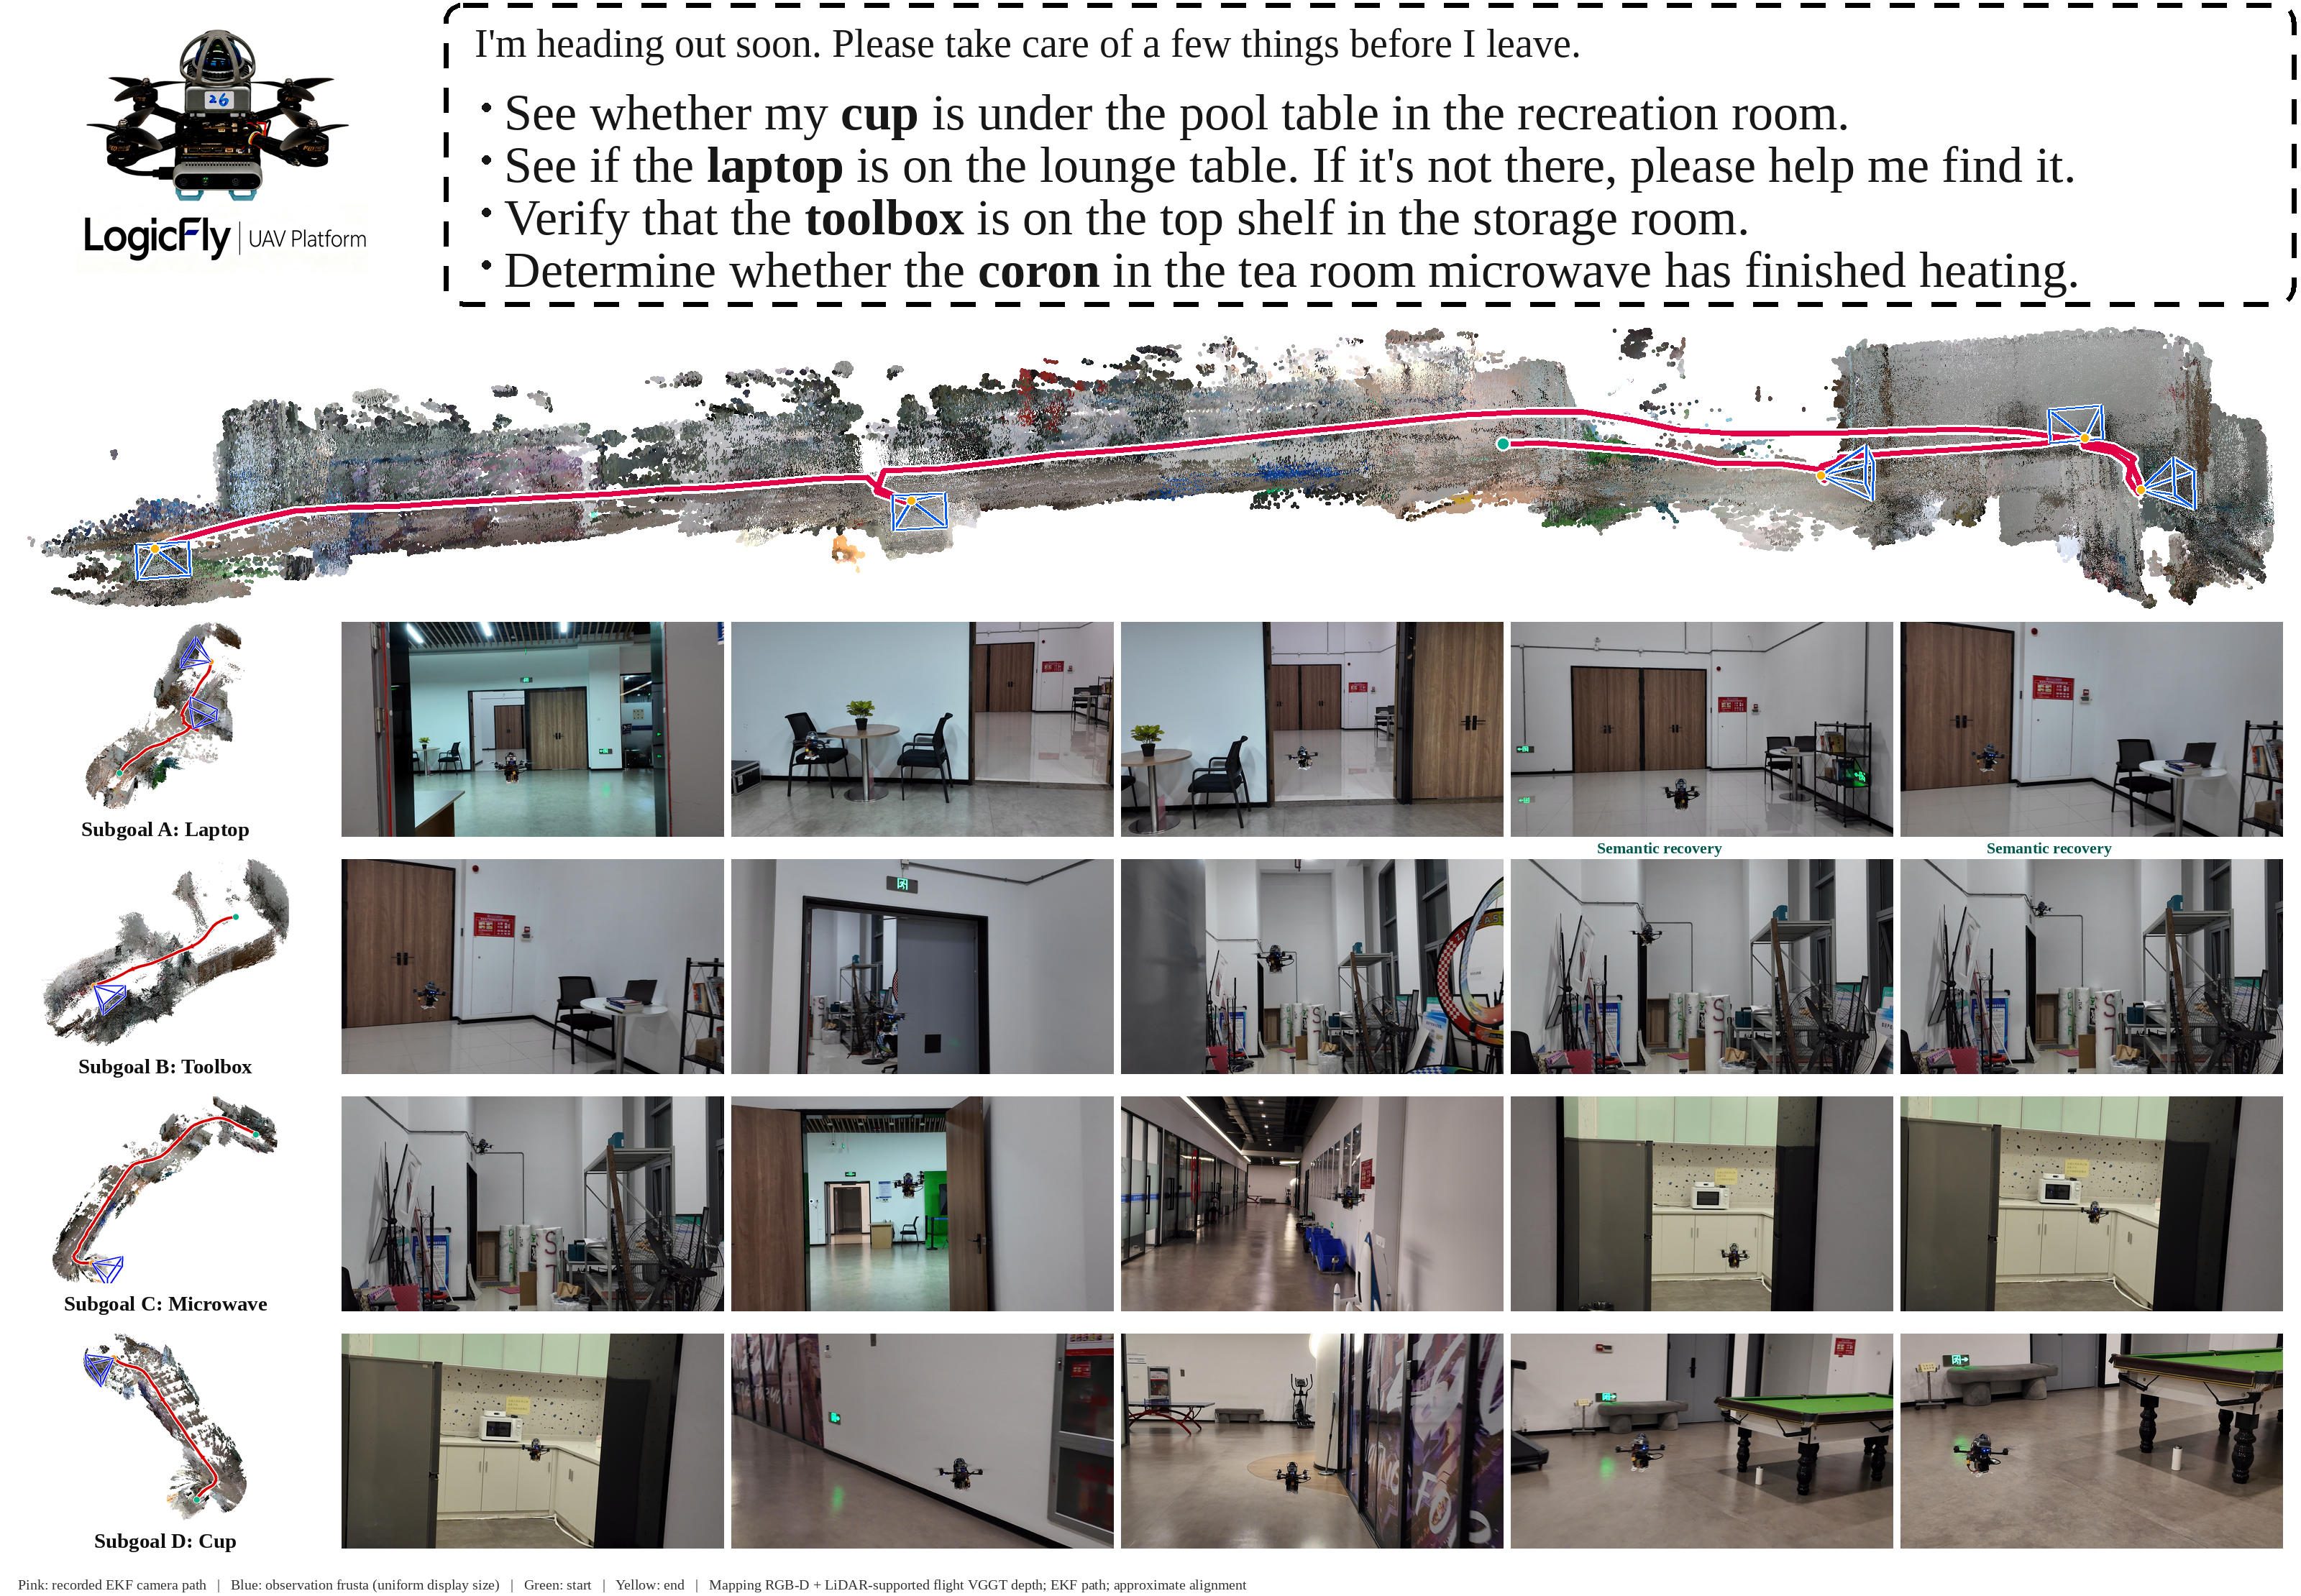
\includegraphics[width=\textwidth]{real_world_execution.png}
\caption{Real-world execution of a single multi-task language instruction by LogicFly. The global reconstruction shows the continuous recorded camera trajectory and observation frusta. Each row pairs a local reconstruction with third-person views of laptop search and recovery, toolbox verification, microwave inspection, or cup verification. Reconstructions fuse VGGT depth with prior mapping RGB-D and LiDAR support; trajectories use onboard EKF odometry with approximate video alignment.}
\label{fig:real-world-main}
\end{figure*}

\section{Introduction}
Indoor aerial robots can support repeated visual inspection, inventory checks, and object search across rooms and floors. These applications require more than reaching an isolated destination: a request may specify several observations, require one check before another, and prescribe a fallback if an expected object is absent. Long-horizon navigation therefore involves deciding what to inspect, where to observe it, and when new evidence should change the remaining mission. Efficient coordination matters because unnecessary travel consumes flight time and delays completion of the overall request.

Many recurring deployments allow the environment to be surveyed before individual tasks arrive. Homes, offices, and managed facilities are repeatedly accessible, and their large-scale geometry often changes more slowly than the objects of interest. Reusing a semantic map is consequently a practical operating assumption for this setting. Visual-language maps and hierarchical scene graphs already demonstrate how prior observations can support language-grounded navigation~\cite{huang2023vlmaps,werby2024hovsg}. The central question is how to turn that prior knowledge into efficient, observation-driven execution when instructions contain multiple interacting requirements and the stored semantics may be incomplete.

Three gaps motivate our formulation. \emph{First, a destination or fixed subgoal list does not fully express task logic.} Conventional VLN benchmarks established instruction following and continuous navigation~\cite{anderson2018r2r,krantz2020vlnce}, and long-horizon VLN extends these settings to sustained multi-stage execution~\cite{song2024lhvln}. For inspection requests, however, mandatory precedence, freely reorderable checks, and conditional alternatives must be distinguished: imposing an unnecessary order wastes travel, whereas ignoring a required order changes the task. \emph{Second, semantic task grounding does not uniquely determine an observation pose.} Scene-graph planners connect language to spatial goals~\cite{rana2023sayplan,dai2024osgp}, but an aerial robot can inspect the same region from different heights and directions. Selecting a pose independently for each task can make the combined route unnecessarily long, and proximity to an object does not ensure visibility. \emph{Third, negative evidence has different meanings at different scales.} Missing an object in one image may justify another view, while exhausting a location may justify searching elsewhere. Treating every missed detection as task failure, or treating every fallback as unrestricted search, loses this distinction.

We address these issues with \textbf{LogicFly}, which separates reusable map construction from task execution. The first stage organizes measured geometry and semantic observations into floors, rooms, and object instances. The second stage represents the request as a Conditional Partial-Order Task Graph (CPTG), generates task-conditioned observation poses, and applies Joint Task--Viewpoint Planning (JTVP) to a bounded set of currently executable tasks. Following each observation, an explicit recovery policy determines whether to retry locally, search another region, or resolve the task and evaluate its conditional rules. This design connects logical progress to geometric observation opportunities without committing the whole mission to an order before its outcomes are known.

Our contributions are:
\begin{itemize}
\setlength{\itemsep}{2pt}
\setlength{\parsep}{0pt}
\item A conditional partial-order execution model that separates precedence, outcome-triggered branches, and within-task recovery, while retaining distinct search anchors and verification targets.
\item A rolling joint planner that couples task ordering with three-dimensional observation-pose selection, using finite candidate sets, visibility scores, and collision-checked travel costs.
\item An evidence-driven execution mechanism that distinguishes local misses from terminal outcomes and updates regional search confidence using newly observed coverage.
\end{itemize}
Qualitative Habitat examples illustrate multi-target execution, recovery after negative observations, and conditional task activation. Physical UAV experiments demonstrate these closed-loop capabilities through online target recognition, conditional task execution, local viewpoint retries, and cross-room recovery search. Section~\ref{sec:evaluation} presents the experimental settings and examples.

% Queue the overview early so it can precede the method figures.
\begin{figure*}[t]
\centering
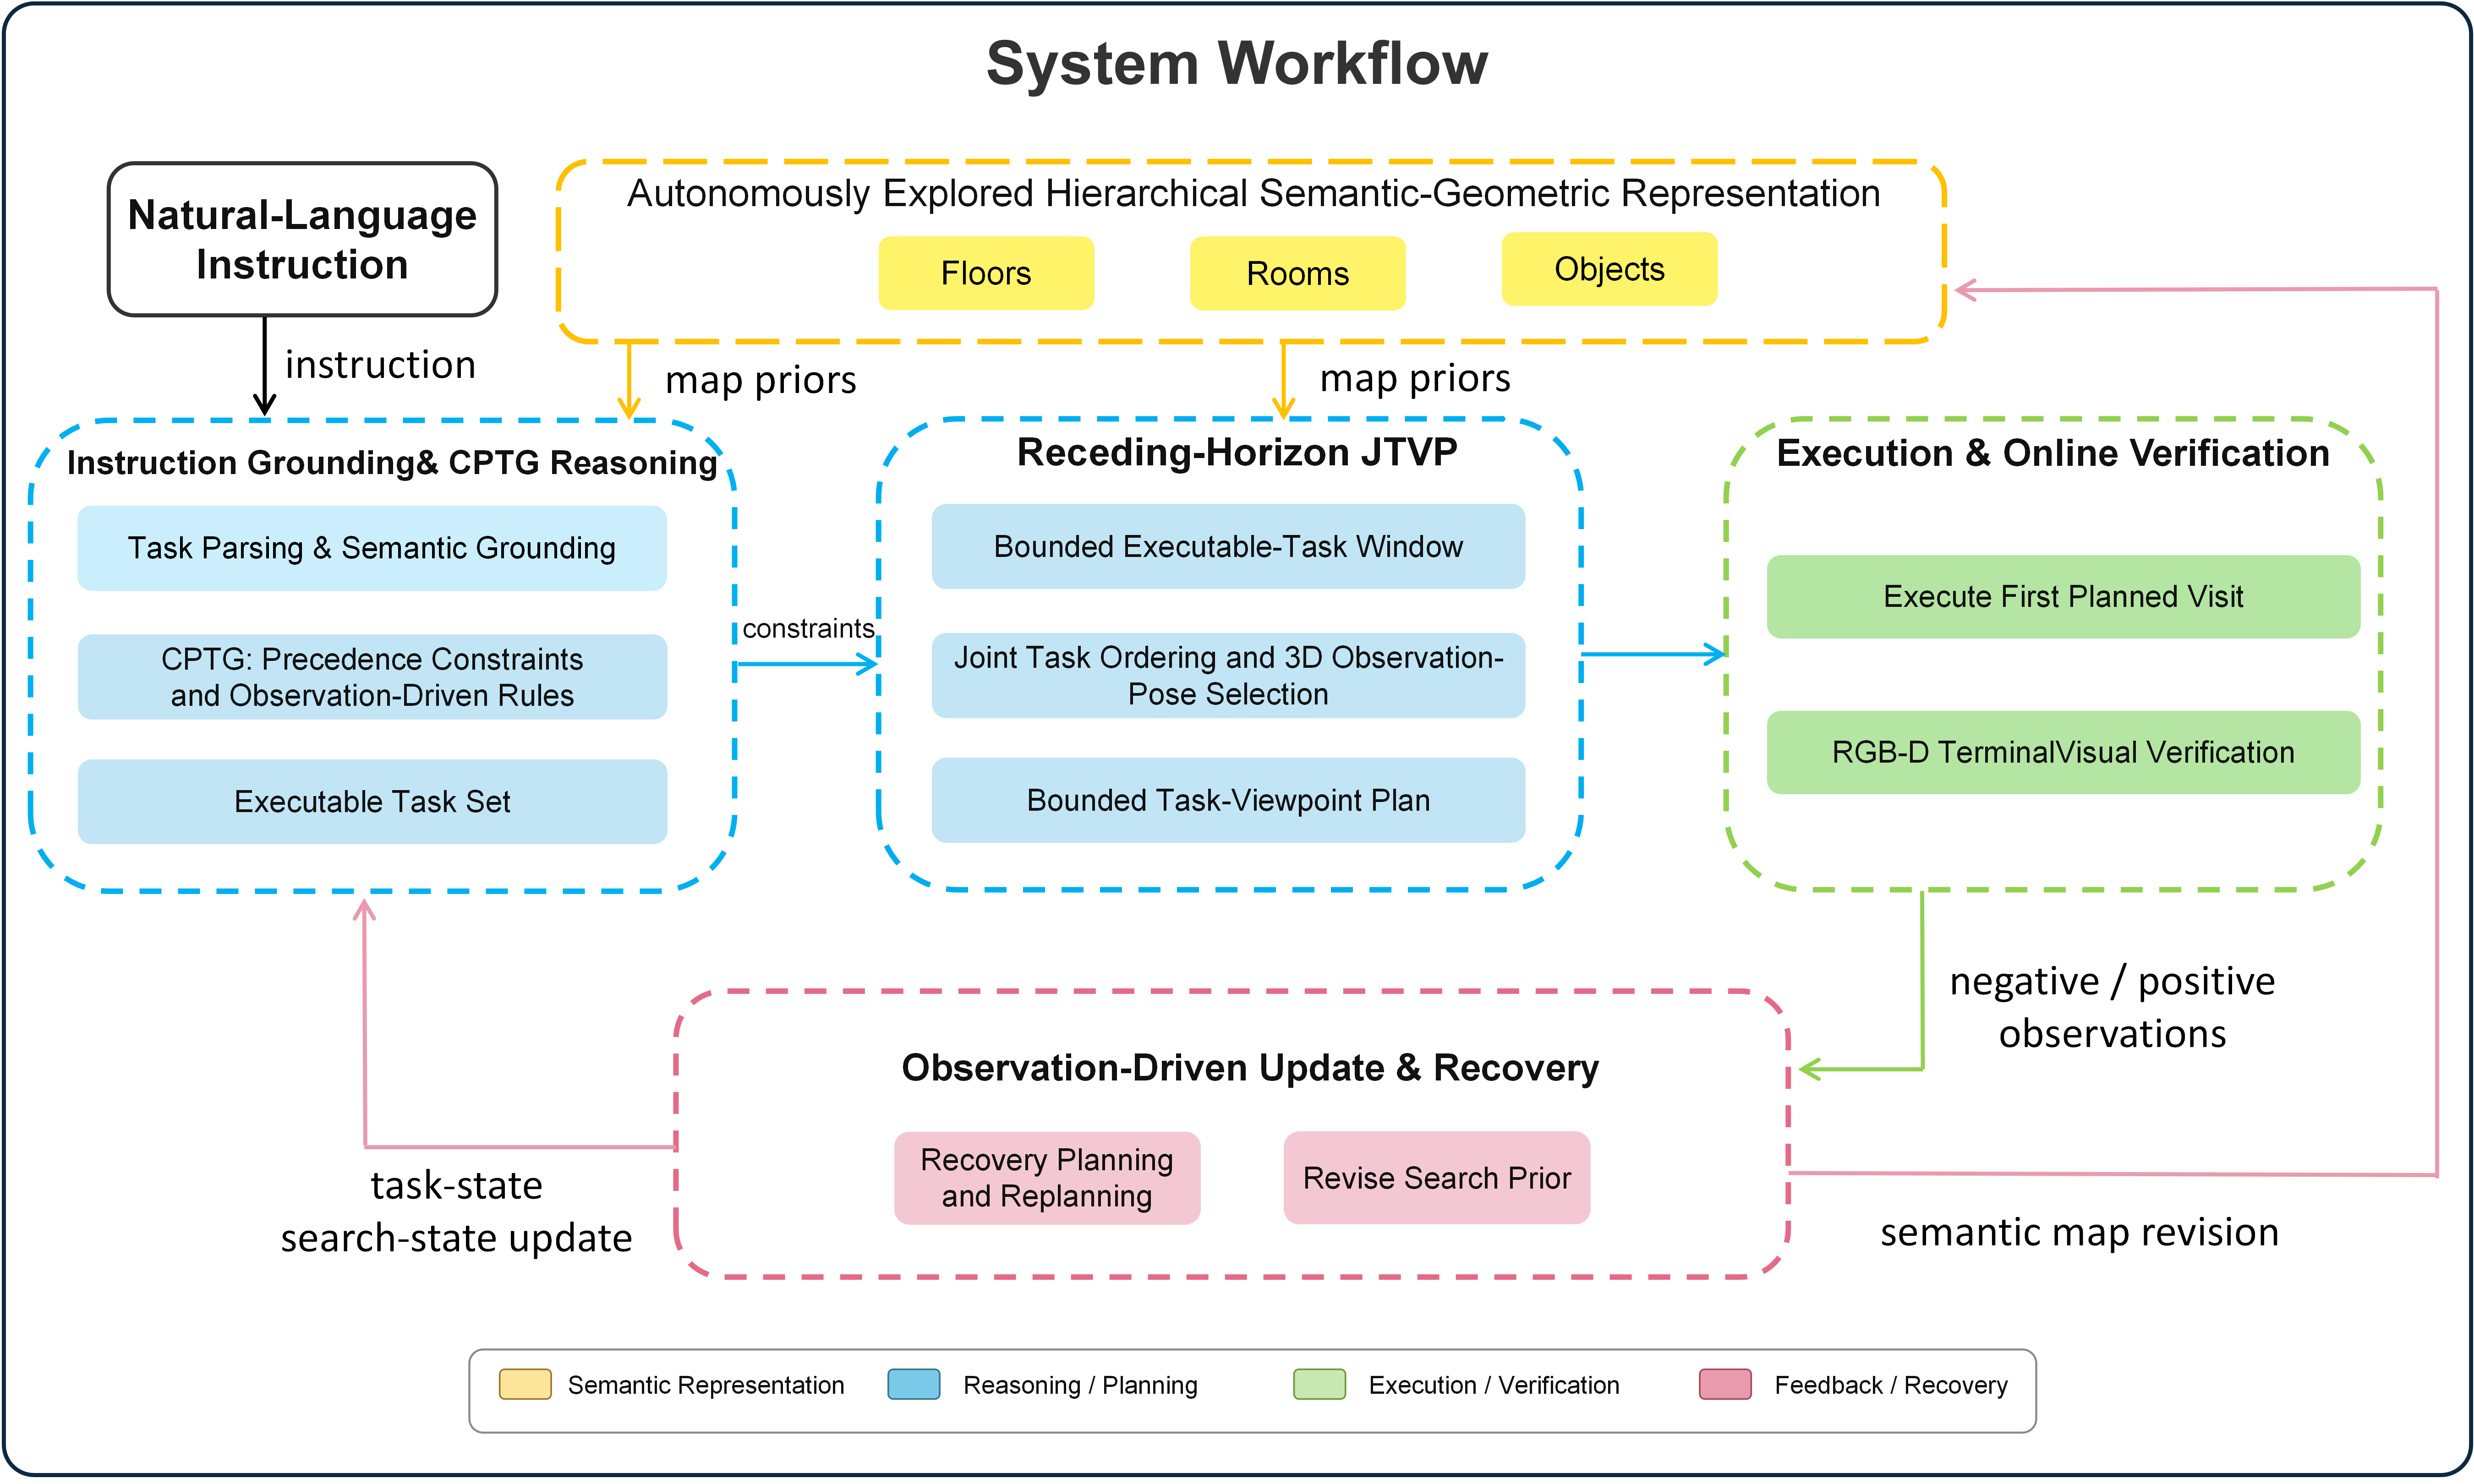
\includegraphics[width=\textwidth]{system_overview.png}
\caption{LogicFly pipeline. Exploration and semantic mapping provide reusable spatial priors. A language request is represented as a CPTG; task-conditioned views and collision-aware costs support rolling JTVP. Observations update task and search states before replanning. The physical deployment is described in Section~\ref{sec:realworld}.}
\label{fig:overview}
\end{figure*}

\section{Related Work}
\subsection{From Instruction Following to Persistent Spatial Memory}
R2R established visually grounded route following~\cite{anderson2018r2r}, while VLN-CE moved execution from a predefined navigation graph into continuous environments~\cite{krantz2020vlnce}. These developments improve the connection between language and motion, but a single episode need not capture the repeated use of a building. Iterative VLN addresses experience reuse across successive instructions~\cite{krantz2023ivln}, and LH-VLN emphasizes consistency across extended subtask sequences~\cite{song2024lhvln}. Together, they motivate persistent memory and longer planning horizons. Our setting additionally requires explicit freedom among unordered tasks and explicit rules for activating alternatives after observations.

VLMaps grounds open-vocabulary and spatial language directly in a reconstructed map~\cite{huang2023vlmaps}. ConceptGraphs organizes observations into object-centric 3D scene graphs~\cite{gu2024conceptgraphs}, and HOV-SG adds floor--room--object hierarchy and cross-floor navigation~\cite{werby2024hovsg}. This progression makes large scenes easier to query, but a grounded object or region still leaves the robot's camera pose and the order of multiple inspections to be chosen. LogicFly builds on this semantic hierarchy to jointly select observation poses and the order of multiple tasks.

\subsection{Structured Task Planning and Observation Geometry}
SayPlan combines hierarchical scene-graph search with classical planning and feasibility feedback, enabling language-conditioned plans in large multi-room environments~\cite{rana2023sayplan}. OSGP gives temporal constraints a formal representation through an LTL automaton and performs optimal hierarchical search over a metric--semantic graph~\cite{dai2024osgp}. These works establish that structured task reasoning can be combined with geometric costs. Our distinction is the finite planning state: each task can have several admissible camera poses, and the planner chooses the task sequence and those poses together. This formulation couples task sequencing with observation geometry within a rolling planning window.

Continuous trajectory optimization addresses a complementary problem. MINCO provides a compact trajectory representation for smooth multicopter motion under geometric and dynamic constraints~\cite{wang2022minco}. AirHunt further connects VLM semantics to continuous aerial object-navigation planning~\cite{chen2026airhunt}. These developments motivate separating continuous trajectory optimization from discrete task planning. LogicFly concentrates on coordinating multiple logically related observation tasks; its discrete task--viewpoint objective uses a geometric travel estimate, and trajectory optimization follows the selected visits.

\subsection{Language-Based Decisions and Closed-Loop Feedback}
NavGPT uses language-model reasoning over observations and action history~\cite{zhou2024navgpt}. MapGPT supplements local observations with an online topological map and adaptive multi-step planning~\cite{chen2024mapgpt}; SpatialNav uses a scene graph acquired before task execution to provide global spatial context~\cite{zhang2026spatialnav}. VLN-Zero similarly separates exploration from deployment and reuses cached task-location trajectories~\cite{bhatt2025vlnzero}. Building on prior exploration and structured memory, LogicFly coordinates observation tasks with precedence constraints and outcome-dependent continuations.

Inner Monologue demonstrates that success and environment feedback can revise language-based plans~\cite{huang2023innermonologue}. For the present observation tasks, the remaining issue is how to interpret a failed check without changing the meaning of the instruction. LogicFly assigns explicit semantics to a failed pose, an exhausted search location, and a terminal task outcome. This supports bounded autonomous recovery while keeping a user-specified conditional branch separate from a new search hypothesis.

% Queue the construction overview before its discussion for two-column floats.
\begin{figure*}[t]
\centering
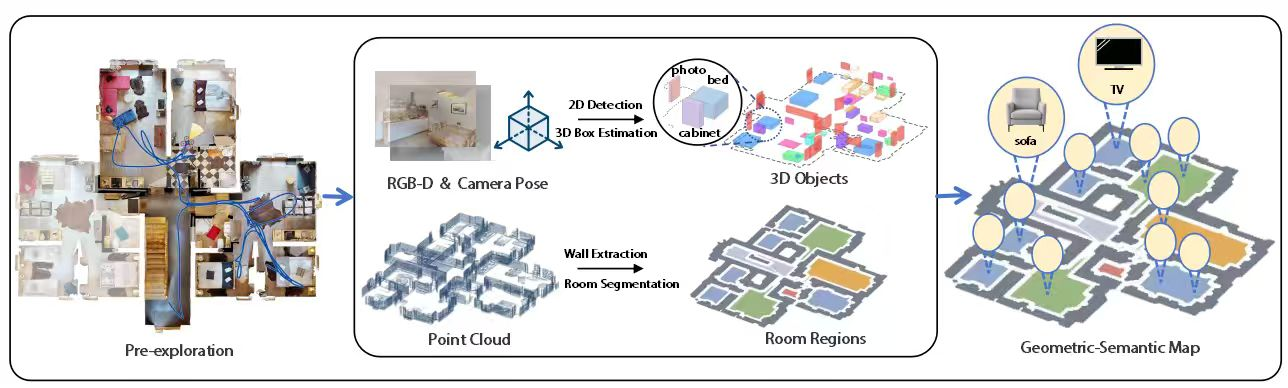
\includegraphics[width=\textwidth]{stage1_mapping_pipeline.jpg}
\caption{First-stage map construction. Autonomous exploration provides RGB-D observations, camera poses, and point-cloud geometry. Object detection and 3D box estimation produce object instances, while wall extraction and room segmentation produce spatial regions. These outputs are integrated into a reusable semantic--geometric map.}
\label{fig:semantic-map-construction}
\end{figure*}

\section{System Overview and Problem Formulation}
\label{sec:overview}
\subsection{Operating Setting and System Pipeline}
We consider one UAV performing navigation and visual observation in a previously surveyed indoor environment. The input is a natural-language request $I$, the current pose $q_0=(x,y,z,\psi)$, and a map $\mathcal M=(\mathcal M_g,\mathcal M_s)$. The geometric map $\mathcal M_g$ distinguishes occupied, observed-free, and unknown space. The semantic map $\mathcal M_s$ associates floors and rooms with object instances, geometry, and confidence. The camera has a fixed, level pitch; position and yaw determine the observation pose. The objective is to complete navigation and visual observation tasks while respecting their logical and geometric constraints.

Figure~\ref{fig:overview} summarizes two stages. During map construction, exploration supplies posed RGB-D observations and measured geometry; semantic fusion and spatial partitioning produce the reusable map. During execution, the instruction is represented as a CPTG whose grounded tasks define possible camera poses. JTVP chooses the next visit using a short lookahead. The executor moves to the selected pose, acquires evidence, and updates task and search states before the next planning step. The occupancy representation determines geometric feasibility, while room labels provide semantic context.

\subsection{Planning State and Objective}
The task representation is $\mathcal G_T=(\mathcal V,\mathcal E_{\mathrm{prec}},\mathcal R_{\mathrm{cond}})$, where the three terms denote tasks, mandatory precedence edges, and conditional activation/skip rules. At decision time $t$, the execution state comprises the robot pose $q_t$, active tasks, resolved outcomes, attempted viewpoints, and regional search confidence. A task may be resolved with a negative outcome; resolution and successful target discovery are therefore different events.

For each task $i$, let $\mathcal Q_i$ contain its feasible observation poses. The planning decision selects a sequence of task--pose pairs from the currently executable tasks, minimizing a combination of travel length, a motion-time proxy, and terminal observation cost. Precedence, branch activation, occupancy, and visibility restrict these choices. The rolling policy commits the first selected visit and reconsiders subsequent visits after new evidence. Optimization is performed over a finite task window and candidate set.

\section{Methodology}
The method connects four operations: constructing reusable spatial priors, representing task logic, jointly selecting tasks and viewpoints, and updating the plan from observations. The semantic map grounds candidate search locations, while the CPTG constrains which tasks can be executed. JTVP then chooses the next observation, and its outcome determines whether to retry, expand the search, or advance the task graph.

\subsection{Reusable Semantic--Geometric Map}
\label{sec:semantic-representation}
The mapping stage supplies spatial priors for later instructions. FALCON~\cite{zhang2024falcon} provides autonomous exploration for collecting RGB-D observations, camera poses, and occupancy evidence. All observations are expressed in a common global frame. The geometric layer retains unknown space as distinct from observed free space, while the semantic layer stores floors, rooms, object labels, 3D boxes, and confidence. Figure~\ref{fig:semantic-map-construction} shows the construction pipeline.

\subsubsection{Object and room semantics}
Text-prompted SAM~3.1, from the SAM~3 model family~\cite{carion2025sam3}, produces object boxes and masks from mapping images. The masks suppress background depth before Boxer~\cite{detone2026boxer} estimates 3D boxes. Multi-view fusion consolidates these observations into object instances, which are associated with spatial room regions by their centers. Room views and associated objects provide evidence for room labels; regions with insufficient evidence remain unknown. The resulting hierarchy supplies anchors for later search, including requests for objects that were not observed during mapping.

\subsubsection{Wall-guided room partitioning}
After exploration, we partition each floor using wall boundaries and observation-supported geometry (Fig.~\ref{fig:room-segmentation}). The procedure first establishes the spatial domain to be partitioned, then extracts interior cores, and finally expands these cores into room regions using marker-controlled watershed segmentation. This formulation exploits the geometric distinction between broad room interiors and narrow connections without requiring room-category predictions during partitioning.

\emph{Wall and observation constraints:} Extracted wall points are projected onto a horizontal grid, and a local morphological closing operation produces a wall-barrier mask $\mathcal W$. Let $\Omega_0$ denote the candidate floor domain. To determine which candidate cells have independent spatial support, we combine four evidence sets: near-horizontal surfaces $\mathcal S_h$, free-space observations at multiple heights $\mathcal S_f$, multi-frame depth-ray coverage $\mathcal S_r$, and recorded trajectory coverage $\mathcal S_t$. The effective partition domain is
\begin{equation}
\Omega=(\Omega_0\setminus\mathcal W)\cap
(\mathcal S_h\cup\mathcal S_f\cup\mathcal S_r\cup\mathcal S_t).
\label{eq:room-domain}
\end{equation}
A candidate cell is retained when at least one support source is available. Walls constrain region boundaries, while the support sets establish which surrounding spaces participate in partitioning. Cells lacking support are excluded from this operation without being classified as exterior or occupied.

\emph{Interior-core extraction:} We compute the Euclidean distance $d(\mathbf x)$ from each cell $\mathbf x\in\Omega$ to the nearest cell outside $\Omega$. Large distances indicate broad interior spaces, whereas small distances occur near domain boundaries and in narrow connections. Core candidates are the connected components of
\begin{equation}
\mathcal C=\{\mathbf x\in\Omega\mid d(\mathbf x)>\tau_c\}.
\label{eq:room-cores}
\end{equation}
Components with area below $A_{\min}$ are discarded; each remaining component receives a distinct marker label. We use $\tau_c=0.45\,\mathrm{m}$ and $A_{\min}=0.04\,\mathrm{m}^2$. Thresholding suppresses narrow connections when their clearance falls below $\tau_c$, allowing adjacent broad interiors to initialize separate regions. These markers are spatial seed regions rather than individual points or semantic room labels.

\emph{Constrained region propagation:} Marker-controlled watershed propagation operates on the negative distance field $-d$ within $\Omega$. Interior cores form the initial basins, and a multi-source priority-queue flood assigns the remaining reachable cells through four-connected neighbors. Propagation minimizes the maximum negative-distance value encountered along a path, so low-clearance connections act as bottlenecks between competing regions. The mask prevents propagation through wall barriers or outside the supported domain. A geometric post-check merges an enclosed region into its sole labeled neighbor when wall support along its boundary is weak and the region does not border unsupported open space. Supported components without a marker remain unassigned. The resulting regions support object association and room naming; the independent 3D occupancy map determines flight feasibility, including obstacles within each region.

\begin{figure*}[t]
\centering
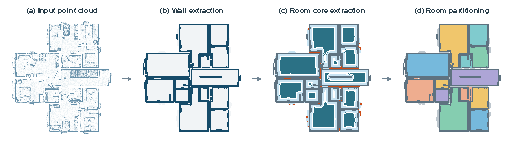
\includegraphics[width=\textwidth]{room_segmentation_en.pdf}
\caption{Wall-guided room partitioning from a recorded floor point cloud. (a) Input measurements. (b) Extracted walls define structural barriers for partitioning. (c) Observation evidence determines the supported domain; connected high-clearance interiors form the cores used to initialize partitioning. Light blue shows supported space outside the cores, orange shows excluded candidates, and dark teal shows interior cores. (d) Marker-controlled watershed propagation within the supported domain, followed by geometric merge checks, produces room regions. Region colors identify partitions; gray denotes supported space without an assigned region. All panels share the same complete floor extent, scale, and orientation.}
\label{fig:room-segmentation}
\end{figure*}

\subsection{Conditional Partial-Order Task Graph}
\label{sec:cptg}
A language model converts the instruction into a CPTG (Fig.~\ref{fig:cptg}). Each node specifies an action, a mapped anchor, a verification target, spatial scope, and search intent. Directed precedence edges encode mandatory order; conditional rules associate an observed outcome with the activation or skipping of other tasks. Task anchors are grounded in the semantic map, and precedence constraints form a directed acyclic graph. Tasks governed by an activation rule remain inactive until its condition is met.

\begin{figure*}[t]
\centering
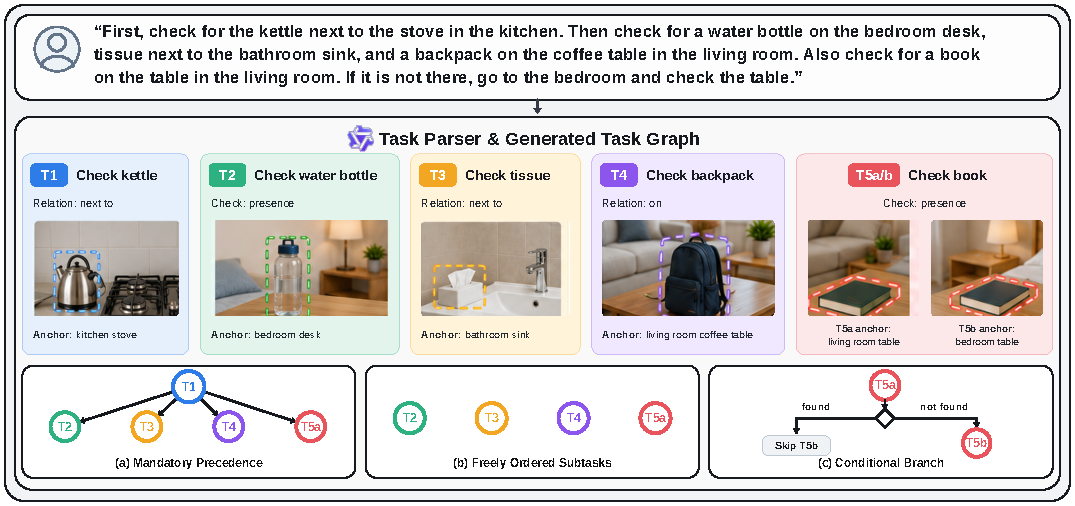
\includegraphics[width=\textwidth]{conditional_task_graph.pdf}
\caption{Language instruction and its CPTG representation. Cards specify verification targets and mapped anchors; relations define search geometry. (a) T1 must resolve before T2--T4 and T5a. (b) These eligible checks have no mutual precedence. (c) A terminal not-found outcome at the living-room table (T5a) activates the bedroom-table check (T5b); a found outcome skips T5b. Scene images are illustrative.}
\label{fig:cptg}
\end{figure*}

\subsubsection{Anchor, target, and intent}
The \emph{anchor} defines where to inspect; the \emph{verification target} defines what to detect. For ``look for a bag under the table,'' the mapped table can anchor the below-table region even when no bag is stored in the map. A relation to another object can disambiguate the intended anchor without replacing it. This separation also determines the meaning of negative evidence: failure to detect the bag does not invalidate the table.

Task intent distinguishes a presence check from a locate-target request. A presence check accepts either discovery or a terminal negative result, whereas a locate-target request requires discovery or a successful explicit fallback. A generic request to keep searching retains the same task and permits autonomous recovery. An explicitly named fallback is represented as a conditional task. These policies are mutually exclusive for a source task, preserving the distinction between an operator's prescribed alternative and an inferred search location.

\subsubsection{Eligibility and outcomes}
Let $\mathcal A_t$ be the active pending tasks and $\mathcal R_t$ the tasks resolved with an outcome. The currently executable set is
\begin{equation}
\mathcal E_t=\{i\in\mathcal A_t:\operatorname{pred}(i)\subseteq\mathcal R_t\}.
\label{eq:eligible}
\end{equation}
A resolved not-found outcome can satisfy a predecessor requirement while triggering a different branch. When a source task terminates, matching rules activate their designated tasks and apply skip rules; inactive alternatives associated with nonmatching rules are skipped. A failed intermediate view does not resolve the source task while its recovery policy still permits another attempt. This preserves the distinction between learning that one camera pose was unproductive and concluding that a conditional fallback should run.

Spatial relations constrain anchor grounding and observation-region construction; observations at the selected pose provide evidence of target presence.

\subsection{Joint Task--Viewpoint Planning}
\label{sec:jtvp}
JTVP converts each executable task into a finite set of camera poses and jointly chooses the visit order and one pose per admitted task. The generation and selection procedures preserve alternatives needed for local recovery while limiting the size of the global discrete optimization.

\subsubsection{Task-conditioned candidate generation}
An anchor and its relation define an observation region, represented by samples $\mathcal P_i=\{s_u\}$ on an object, a support surface, a surrounding neighborhood, or a below-object region. Candidate horizontal positions are sampled over azimuths and stand-off distances. Without an explicit distance constraint, let $R_i$ be half the horizontal diagonal of the region anchor's bounding box and $\alpha_h$ the horizontal field of view (FoV). We sample three center distances
\begin{equation}
D_i(\eta)=\frac{R_i}{\sin(\eta\alpha_h/2)},\qquad
\eta\in\{1,\,0.75,\,0.5\}.
\end{equation}
The bounding circle then subtends a fraction $\eta$ of the horizontal angular FoV. These fixed angular sampling levels provide near, intermediate, and far views while scaling with box size; they do not denote image-pixel coverage or guarantee visibility. Stand-off distances are $d_i(\eta)=D_i(\eta)-R_i$. The intermediate distance is preferred for normal observation, while fine observation prefers the near distance and retains all three rings. Each ring samples 24 azimuths, and candidate yaw faces the region center. Explicit distance constraints override the automatic ring construction. Height, collision, and visibility checks determine feasibility.

For a sampled horizontal position $\bm x$, let $\rho_u=\|\bm x-s_{u,xy}\|_2$ and let $\alpha_v$ denote vertical FoV. For a level camera, vertical inclusion of every region sample gives the height interval
\begin{equation}
\begin{aligned}
h_u&=\rho_u\tan(\alpha_v/2),\\
\mathcal H_i(\bm x)&=\mathcal H_{\mathrm{flight}}\cap
\bigcap_{s_u\in\mathcal P_i}[s_{u,z}-h_u,\ s_{u,z}+h_u].
\end{aligned}
\label{eq:height}
\end{equation}
Here, $\mathcal H_{\mathrm{flight}}$ denotes admissible flight heights. An empty intersection rejects the horizontal sample. Otherwise, the nominal height is chosen closest to the mean region height within the feasible interval. Additional heights can provide finer observation detail; task-specified heights remain subject to geometric and visibility constraints. Equation~\ref{eq:height} controls vertical inclusion before occlusion is considered.

For pose $q=(x,y,z,\psi)$, let $\mathcal V_i(q)$ be the region samples inside both FoV limits and with a valid line of sight. The visibility score is
\begin{equation}
Q_i(q)=\frac{|\mathcal V_i(q)|}{\max(1,|\mathcal P_i|)}.
\label{eq:visibility}
\end{equation}
The generator rejects invalid 3D states and disallowed directional or between-object configurations. For tasks requiring visibility, feasibility is established by visible samples in the observation region, allowing the camera to inspect a region around an occluded anchor center.

Feasible candidates receive a terminal cost
\begin{equation}
\begin{aligned}
C_i^{\mathrm{view}}(q)={}&\beta_d\frac{|d-d_i^{\mathrm{pref}}|}{\ell_0}
+\beta_Q(1-Q_i(q))
+\beta_z\frac{|z-\bar z_i|}{\ell_0}\\
&+\beta_r\frac{d_i^{\mathrm{ref}}}{\ell_0}
+\beta_b\frac{d_i^{\mathrm{between}}}{\ell_0},
\end{aligned}
\label{eq:view-cost}
\end{equation}
where $d$ is stand-off distance, $d_i^{\mathrm{pref}}$ is its preferred value, $\bar z_i$ is mean sample height, $d_i^{\mathrm{ref}}$ is the mapped anchor's horizontal distance to the nearest reference, and $d_i^{\mathrm{between}}$ is the between-reference geometric penalty. The nonnegative weights $\beta_d$, $\beta_Q$, $\beta_z$, $\beta_r$, and $\beta_b$ balance these terms. Inapplicable terms vanish, and $\ell_0$ is a reference length that makes distance penalties dimensionless. The reference-distance term distinguishes anchor hypotheses, while the pose-dependent terms distinguish views of each anchor.

Each physical location hypothesis contributes a compact set of complementary views. Below-object regions first retain the most visible, lowest-cost pose at each feasible azimuth, then maximize angular diversity if pruning is needed. Other regions retain feasible height diversity and favor spatially distinct views with complementary visible samples. This yields $\mathcal Q_i$, with a bounded number of poses per location. Figure~\ref{fig:viewpoint-generation} shows the below-object case.

\begin{figure}[t]
\centering
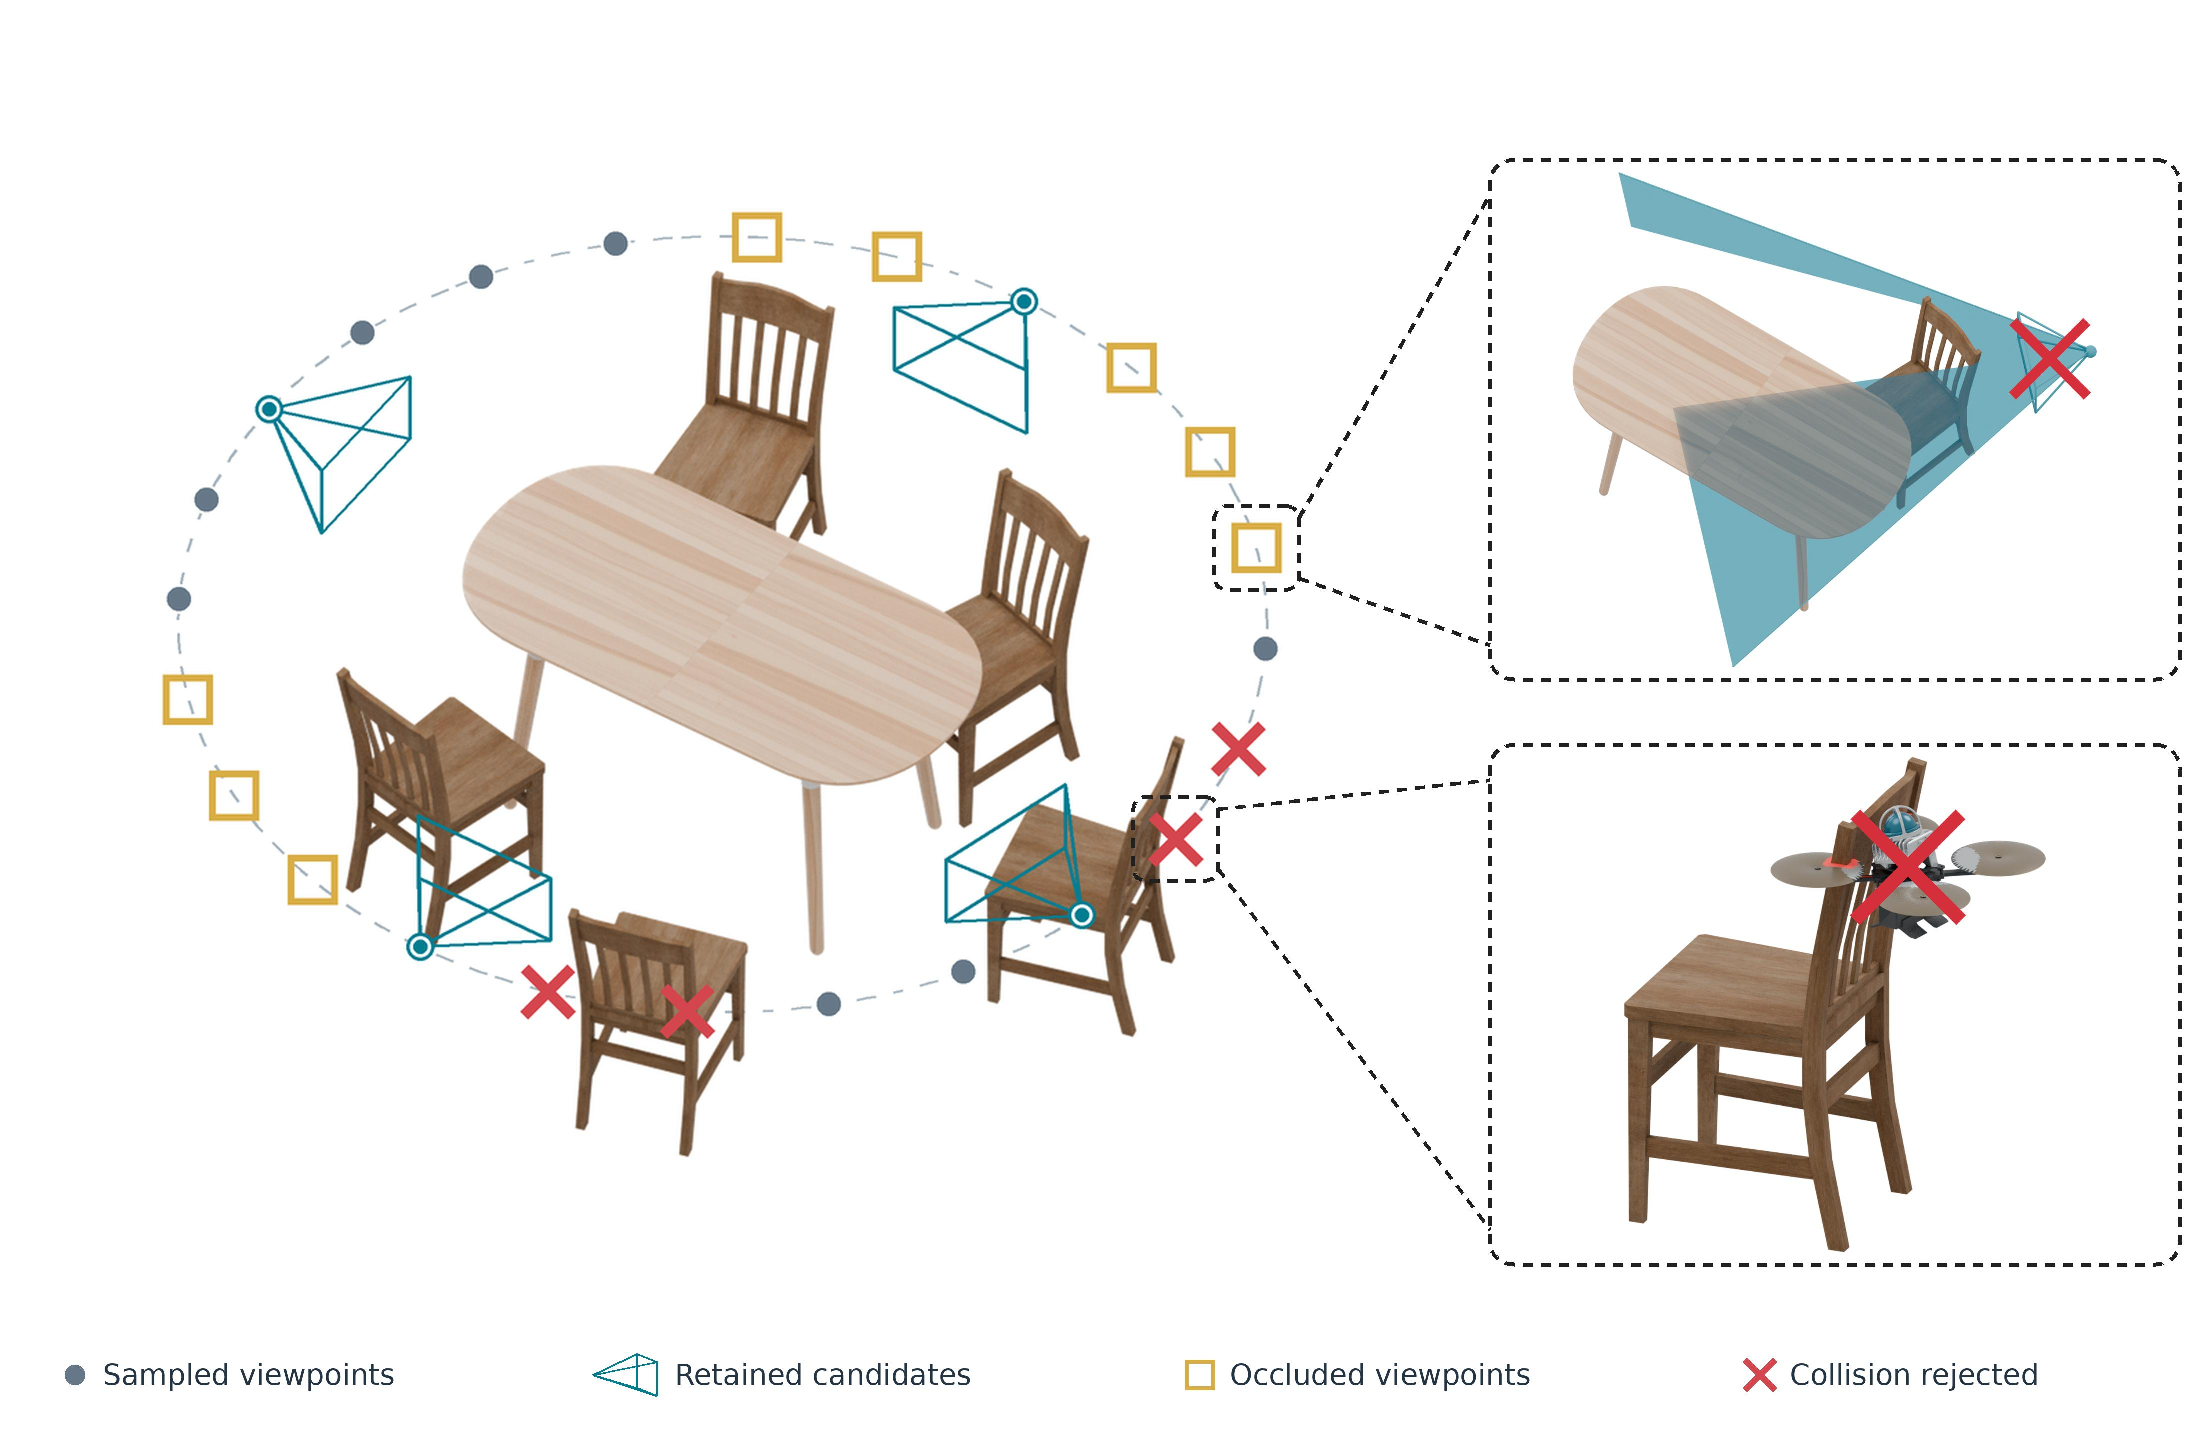
\includegraphics[width=\columnwidth]{viewpoint_generation_en.pdf}
\caption{Candidate viewpoint generation and geometric screening around a dining-table anchor. The main scene shows sampled viewpoints, retained candidates for subsequent planning, occluded viewpoints, and collision-rejected samples. The upper inset illustrates partial field-of-view occlusion by a chair; the lower inset highlights UAV--chair interference. The UAV is enlarged for visual clarity.}
\label{fig:viewpoint-generation}
\end{figure}

\subsubsection{Transition cost}
A$^*$ estimates collision-free travel through observed free space between candidate poses. For a returned path $P_t(q_a,q_b)=\{p_u\}$ and $\Delta\psi_{ab}=\operatorname{wrap}(\psi_b-\psi_a)$, define
\begin{equation}
\begin{aligned}
L_t(q_a,q_b)&=\sum_u\|p_{u+1}-p_u\|_2,\\
\widehat T_t(q_a,q_b)&=\max\left\{
\frac{L_t(q_a,q_b)}{v},\frac{|z_b-z_a|}{v_z},
\frac{|\Delta\psi_{ab}|}{\omega_\psi}\right\}.
\end{aligned}
\label{eq:motion-cost}
\end{equation}
Here, $v$, $v_z$, and $\omega_\psi$ are nominal translational, vertical, and yaw rates. The maximum gives a travel-time proxy for discrete planning. An unreachable transition has infinite cost. For a destination pose belonging to task $i$, the transition score is
\begin{equation}
c_t(q_a,q_b)=\frac{L_t(q_a,q_b)}{\ell_0}
+\eta_T\frac{\widehat T_t(q_a,q_b)}{\tau_0}
+\eta_V C_i^{\mathrm{view}}(q_b),
\label{eq:transition-score}
\end{equation}
where $\tau_0$ is a reference duration for time normalization, and $\eta_T$ and $\eta_V$ balance travel time and observation quality.

\subsubsection{Task window and representatives}
To bound planning cost, executable tasks are ranked by their best Euclidean-distance and terminal-cost estimate, and at most $H$ tasks enter the window $\mathcal W_t$. Views at each physical location are ranked using distance, estimated motion time, and terminal cost. The initial optimization uses the highest-ranked representative at each location. If the complete task window is infeasible, additional representatives are progressively admitted, up to the full candidate set. This adaptive expansion preserves alternatives for feasibility while controlling the number of geometric path queries. Multiple anchor hypotheses contribute separate representatives.

\subsubsection{Subset dynamic program}
Let $\widetilde{\mathcal Q}_{i,t}$ be the admitted poses and $D(S,i,k)$ the minimum cost of visiting task subset $S$ and ending at $q_i^k$. Initialization and transitions are
\begin{equation}
\begin{aligned}
D(\{i\},i,k)&=c_t(q_t,q_i^k),\\
D(S\cup\{j\},j,\ell)&=\min_{i\in S,k}
\bigl[D(S,i,k)+c_t(q_i^k,q_j^\ell)\bigr].
\end{aligned}
\label{eq:subset-dp}
\end{equation}
Initialization requires $\operatorname{pred}(i)\subseteq\mathcal R_t$. A transition requires $j\notin S$, $\operatorname{pred}(j)\subseteq\mathcal R_t\cup S$, and a finite path cost. Unavailable states have infinite value. Backtracking from $\min_{i,k}D(\mathcal W_t,i,k)$ yields the visit order and observation poses.

For $m$ admitted tasks and at most $K$ admitted candidates per task, the recurrence has $O(2^m m^2K^2)$ transition complexity, excluding geometric path search. The recurrence yields the minimum-cost sequence over the admitted task window and pose sets. The robot executes the first visit and then replans using the updated observations. During local recovery, the remaining views of the current location are prioritized to avoid repeatedly leaving an unresolved search region.

\begin{figure*}[t]
\centering
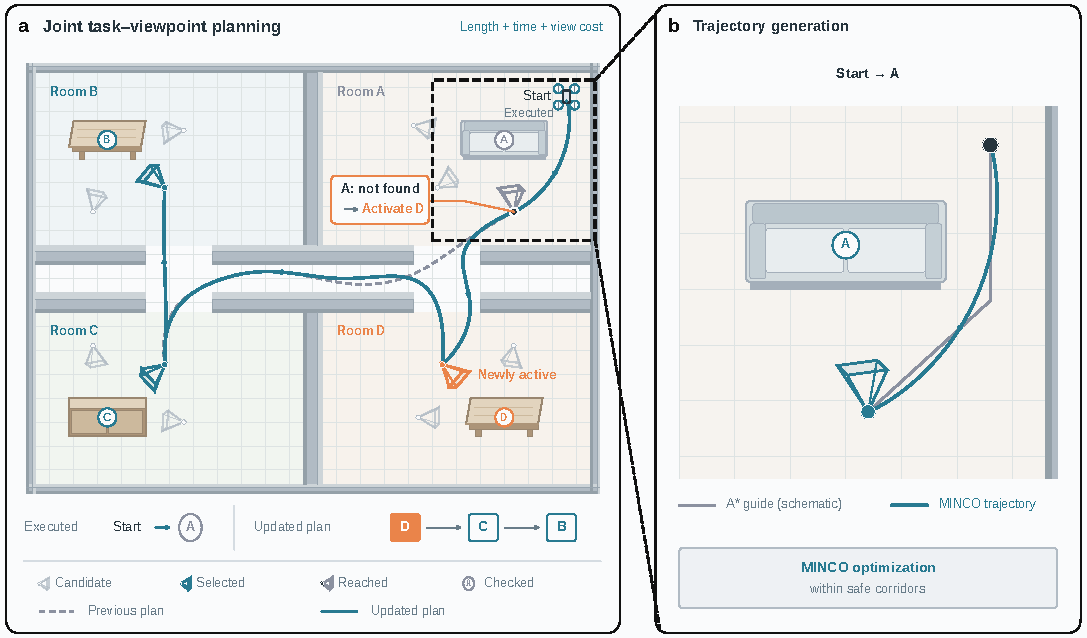
\includegraphics[width=\textwidth]{joint_task_viewpoint_planning_en.pdf}
\caption{Joint task--viewpoint planning and trajectory generation. (a) Each room has one illustrative task anchor and several candidate views. After the Start $\rightarrow$ A visit, a terminal not-found outcome activates D and changes the remaining order from C $\rightarrow$ B to D $\rightarrow$ C $\rightarrow$ B. Grey dashed curves show the previous plan; teal shows the updated route and executed prefix. Faint and bold wireframes indicate candidate and selected views, and orange marks the newly activated task. (b) The dashed box identifies the enlarged region: an A$^*$ guide (grey, simplified for display) supports safe-corridor construction and MINCO optimization (teal). This is a mechanism illustration with a computed trajectory.}
\label{fig:jtvp-illustration}
\end{figure*}

\subsection{Execution, Recovery, and Semantic Updates}
\label{sec:recovery}
\label{sec:execution}
The execution loop associates each visit with an observation and a task-policy decision. Figure~\ref{fig:semantic-recovery} illustrates how local reinspection and semantic recovery preserve the cushion-search objective within a multi-object inspection mission.

\begin{figure*}[t]
\centering
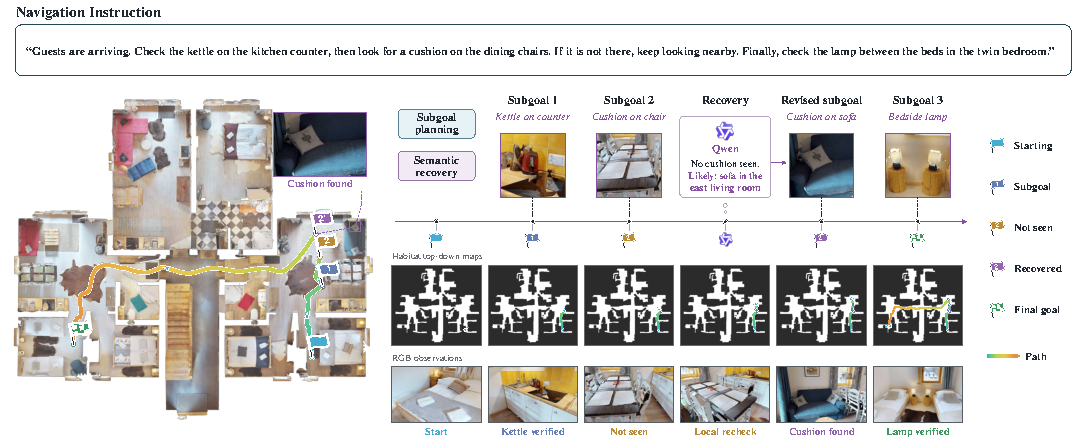
\includegraphics[width=\textwidth]{semantic_recovery_en.pdf}
\caption{Illustration of semantic recovery within a multi-object inspection task. The sequence checks a kettle on the kitchen counter, searches the dining chairs for a cushion, and checks a bedside lamp. After local reinspection yields no cushion observation, the recovery module proposes the sofa in the eastern living room as an alternative search anchor. The cushion is then located, and the mission continues to the bedroom. Flags associate key observation poses with the trajectory, top-down maps, and RGB views.}
\label{fig:semantic-recovery}
\end{figure*}

\subsubsection{Trajectory generation and observation}
The selected geometric route is converted into a smooth, collision-checked trajectory toward the next observation pose. Habitat execution uses cubic B-spline smoothing, while physical flight uses MINCO~\cite{wang2022minco} within safe corridors, as illustrated in Fig.~\ref{fig:jtvp-illustration}(b). Trajectory optimization refines continuous motion after the discrete task--viewpoint decision. At the selected pose, the robot acquires an RGB-D observation and evaluates the task's verification target.

Text-prompted SAM~3.1 provides category detections for online verification. Depth and camera pose project detections into the global frame, where spatial association checks their consistency with mapped objects or accumulated novel-instance tracks. A positive visual outcome requires both a target-category detection and geometric confirmation. Spatial relations determine where to search, while the visual check establishes category presence and geometric consistency; relation-specific truth is not a separate termination criterion. The resulting observation updates the task state and determines the next planning action.

\subsubsection{Three levels of negative evidence}
A \emph{pose-level miss} leaves the task unresolved while alternative local views remain. These views provide different observation directions around the same anchor. A \emph{location-level exhaustion} occurs when the local candidate set is exhausted or the local search limit is reached. For a locate-target request that permits autonomous recovery, the missing target, instruction, failed anchors, and scene inventory condition alternative room--anchor--region hypotheses. Grounding these hypotheses in mapped entities yields new search regions and feasible camera poses. Search continues within a bounded set of locations, with room-level alternatives available when anchor-specific views are exhausted.

A \emph{terminal task outcome} is emitted only when the target is found or no permitted continuation remains. A terminal not-found indicates that the permitted search locations and viewpoints have been exhausted without confirming the target. The task intent determines whether it is an acceptable presence-check result, an unresolved locate-target task, or the trigger for an explicit fallback. Only then does CPTG evaluate its conditional rules.

\subsubsection{Coverage-aware search confidence}
For a semantic search region $r$, let $b_r\in[0,1]$ denote its search confidence, $\mathcal P_r$ its spatial samples, $U_r$ the samples already covered, and $V(q)$ the samples with an unobstructed ray from pose $q$. The ratio $Q_r(q)=|V(q)|/\max(1,|\mathcal P_r|)$ measures line-of-sight coverage. It is a geometric search proxy; camera FoV is enforced during candidate generation through Eq.~\ref{eq:visibility}. A negative observation gives
\begin{equation}
\begin{aligned}
\Delta Q_r(q)&=\frac{|V(q)\setminus U_r|}{\max(1,|\mathcal P_r|)},\\
b_r^+&=b_r[1-\rho\,\Delta Q_r(q)Q_r(q)],\\
U_r^+&=U_r\cup V(q),
\end{aligned}
\label{eq:belief}
\end{equation}
where $\rho\in[0,1]$ controls the strength of negative evidence. A positive observation sets $b_r^+=1$. Because confidence decreases only with newly covered samples, repeated observations of the same region do not accumulate redundant negative evidence. The bounded confidence score prioritizes subsequent search regions. Semantic-region candidates are ranked by
\begin{equation}
C_r^{\mathrm{search}}(q)=\lambda_L\bar L_r^{\mathrm{cover}}+\lambda_Q[1-Q_r(q)]+\lambda_b(1-b_r),
\label{eq:search-cost}
\end{equation}
where $\bar L_r^{\mathrm{cover}}$ is the normalized region-coverage travel estimate and the nonnegative weights balance travel, coverage, and semantic confidence. Initial confidence reflects the relevance of each recovery hypothesis. This cost replaces the ordinary terminal cost for semantic-region candidates, directing subsequent observations toward accessible regions that remain plausible.

\subsubsection{Object confidence and new instances}
When the mapped object is also the verification target, its confidence increases toward one after a positive observation and decreases after a negative observation. These updates are $p^+=p+\alpha_+(1-p)$ and $p^+=\alpha_-p$, with $\alpha_+,\alpha_-\in(0,1)$. Failure to find a different target near a surrogate anchor does not reduce the anchor's existence confidence. Unmatched same-category RGB-D detections are associated across observations, and consistently supported tracks are added as new instances after execution. Regional confidence supports the ongoing search, while the revised object map supplies priors for later missions.

The complete loop thus grounds the instruction, constructs and filters views, selects a task--pose visit, executes it, and updates the appropriate evidence level. It continues local search when warranted and returns to global scheduling after task resolution or a change of search location. This preserves task logic while allowing geometric choices to respond to observations.

\section{Evaluation}
\label{sec:evaluation}
We examine navigation and visual observation in Habitat and physical UAV experiments. The simulation examples cover reorderable checks, recovery after unsuccessful observations, and explicit conditional branches.

% Queue the wide execution strip near the evaluation entry for the next page.
\begin{figure*}[t]
\centering
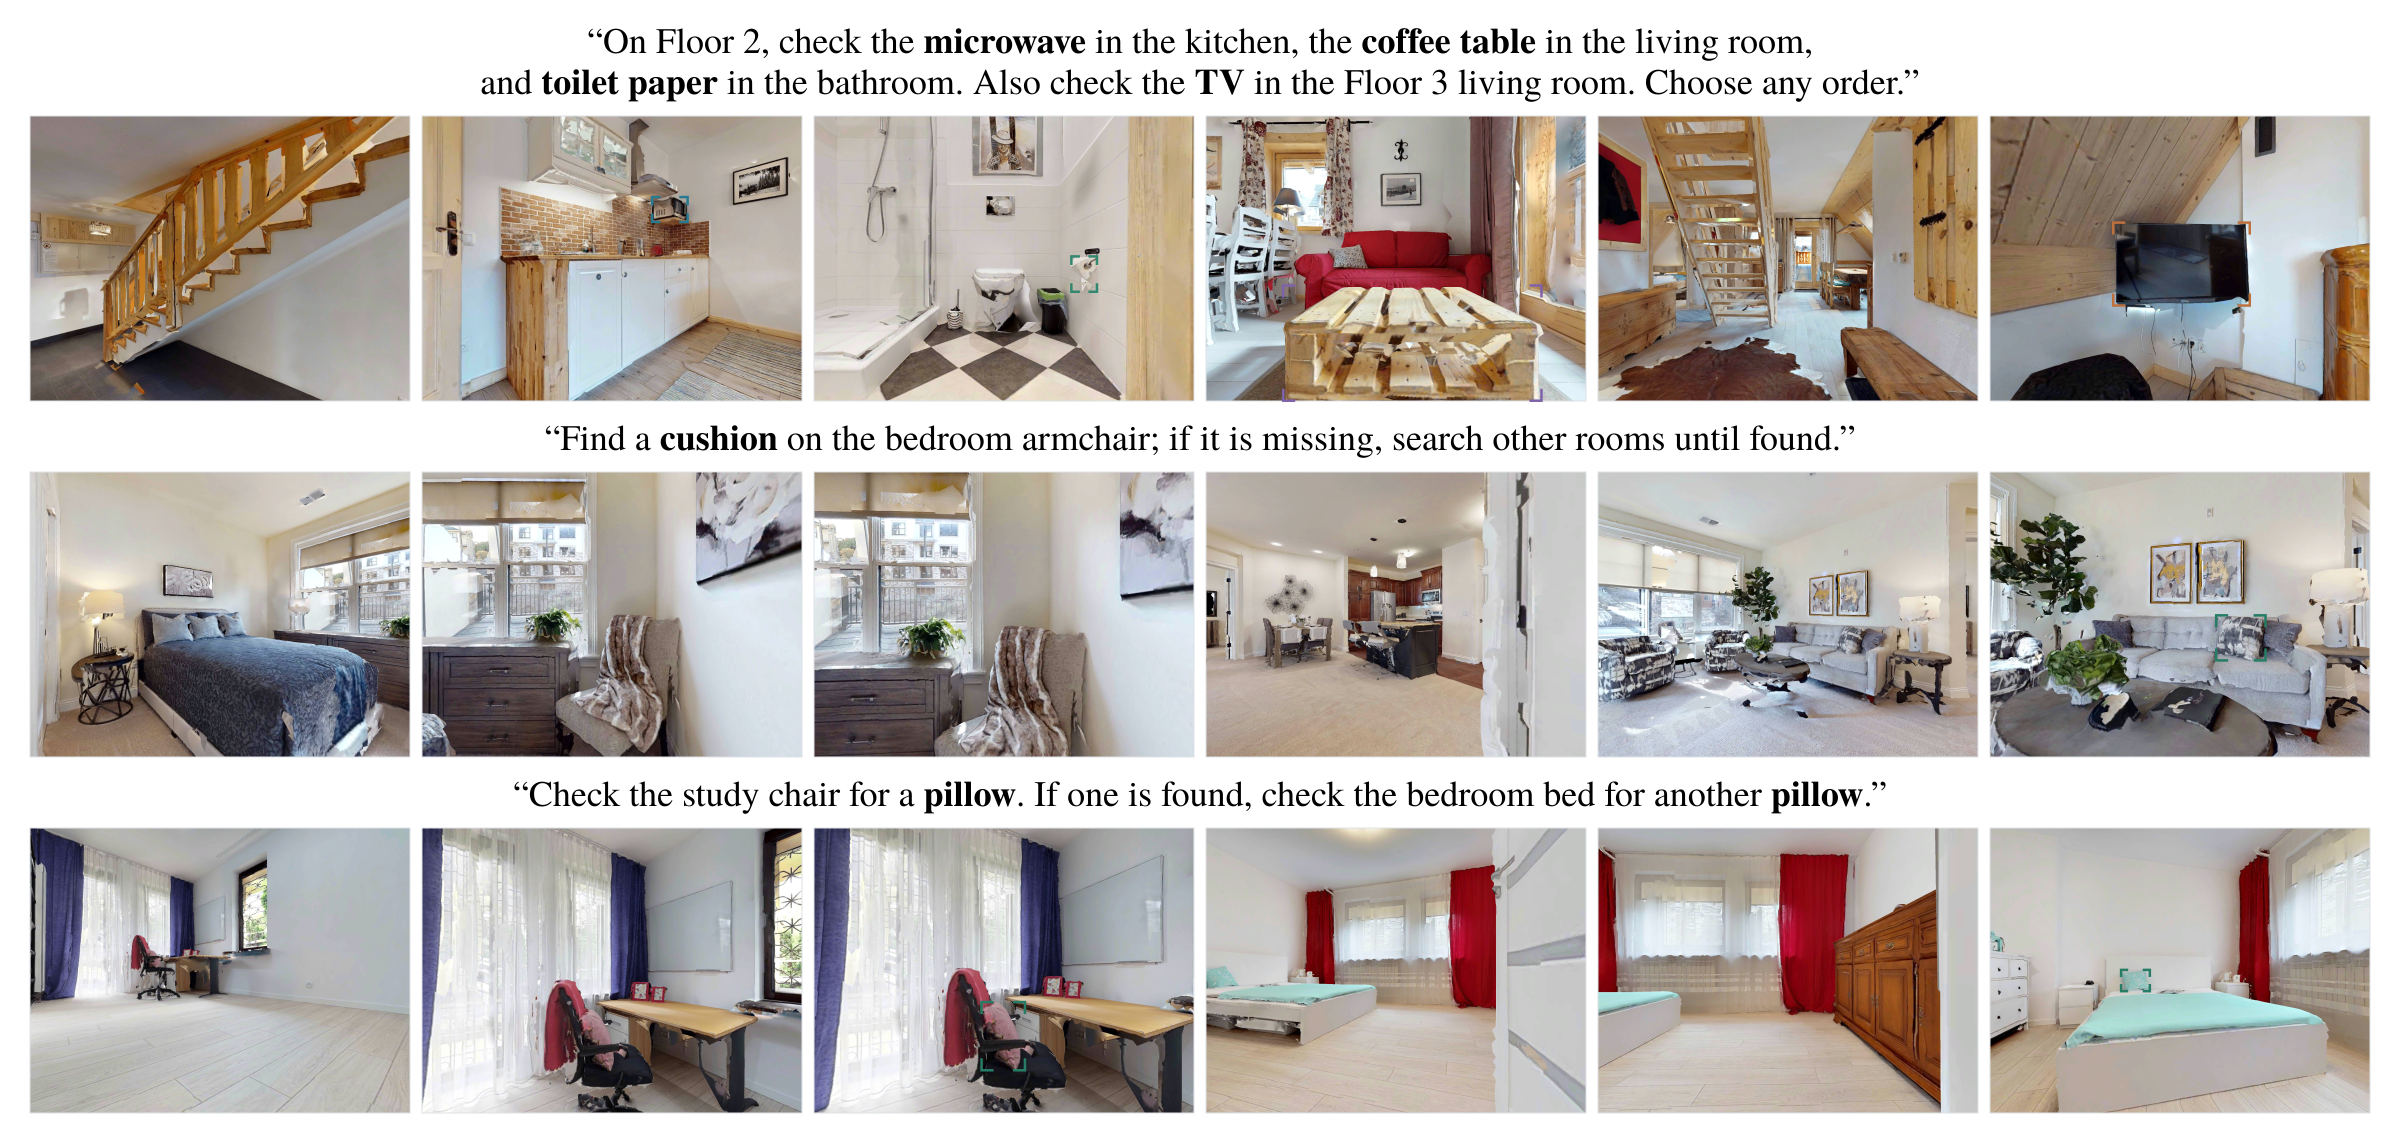
\includegraphics[width=\textwidth]{habitat_long_instruction_en.png}
\caption{Simulation visualizations. Each row shows a navigation episode, with the language instruction above representative first-person UAV keyframes along the trajectory.}
\label{fig:habitat-execution}
\end{figure*}

\subsection{Experimental Setup}
\label{sec:implementation}
Simulation uses Habitat~\cite{savva2019habitat} with HM3D indoor scenes~\cite{ramakrishnan2021hm3d}. Each episode combines a language-specified task, a preconstructed semantic--geometric map, and RGB-D observations acquired during navigation. The scenes contain multiple rooms and, where applicable, multiple floors. The qualitative examples examine how the robot coordinates observations, responds to an unsuccessful search, and follows conditional task requirements.

\subsection{Benchmark and Metrics}
The task families include single-target navigation, ordered and reorderable multi-target checks, conditional alternatives, and recovery when an expected target is missing. Task success requires the requested terminal outcomes while respecting precedence and activated branches. Reaching an anchor alone does not satisfy a visual check. A bounded negative outcome can resolve a presence check, whereas a locate-target request remains unsuccessful without discovery or its prescribed fallback.

We define trajectory length (TL) from the executed 3D path and full-task success rate (SR) over all attempted episodes. For episodes with a valid branch- and order-consistent reference route, success weighted by path length is
\begin{equation}
\mathrm{SPL}=\frac{1}{|\mathcal D_g|}\sum_{e\in\mathcal D_g}
S_e\frac{L_e^{\mathrm{ref}}}{\max(L_e^{\mathrm{ref}},L_e)},
\label{eq:spl}
\end{equation}
where $L_e$ and $L_e^{\mathrm{ref}}$ denote the executed and reference route lengths, respectively. The set $\mathcal D_g$ contains episodes with a defined geometric goal and a valid reference route, and $S_e\in\{0,1\}$ denotes full-task success. Reference routes obey the same precedence and activated-branch constraints as the evaluated mission. Absence checks without a geometric goal are assessed by their required terminal outcome and excluded from SPL. Execution time and task-level outcomes complement path efficiency.

\subsection{Qualitative Execution in Habitat}
\label{sec:qualitative}
Figure~\ref{fig:habitat-execution} illustrates execution across different indoor scenes. For multi-target instructions, the robot visits observation locations across rooms and floors. When an expected object is not observed, it retries alternative local views before extending the search to another room, retaining the original search objective. For conditional instructions, a successful observation activates the subsequent task specified by the instruction. These behaviors illustrate how task logic and visual feedback jointly guide mission progress, while distinguishing recovery within an ongoing task from activation of a new task.

\subsection{Comparison with Existing Methods}
\label{sec:comparison}
\emph{Results to be added.}

\subsection{Ablation Studies}
\label{sec:ablation}
\emph{Results to be added.}

\subsection{Physical UAV Experiments}
\label{sec:realworld}
The deployment platform comprises a quadrotor, a Jetson Orin NX, a PX4 flight controller, a Livox Mid-360 LiDAR, and an Intel RealSense D435 RGB-D camera. LiDAR--inertial localization uses the FAST-LIO family~\cite{xu2021fastlio} and aligns the vehicle with the mapped environment.

The physical experiments cover cross-room flight, online target recognition, conditional task activation, local viewpoint retries, and recovery search across rooms. During execution, visual observations update the task state: an unsuccessful local observation leads to another viewpoint, while exhaustion of the local search prompts exploration of an alternative room. For instructions with conditional requirements, the observed outcome determines whether a subsequent task becomes active. These experiments exercise the connection between task logic, viewpoint selection, perception, and physical motion.

Figure~\ref{fig:real-world-main} presents a multi-room execution example with the UAV route and camera observations. The reconstruction provides spatial context, while the observation sequence shows the views acquired along the flight.

\section{Conclusion}
LogicFly addresses long-horizon language-guided aerial navigation in environments where a reusable semantic map can be constructed before task execution. Its CPTG distinguishes precedence and explicit conditional alternatives, while JTVP couples task ordering with three-dimensional observation-pose selection. A staged recovery loop interprets negative observations at the pose, location, and task levels and updates search confidence from newly observed coverage. Together, these mechanisms connect semantic priors to observable goals and evidence-driven task progress.

The Habitat examples illustrate multi-room checks, task-preserving recovery, and outcome-triggered activation. Physical UAV experiments demonstrate the corresponding closed-loop behaviors, including online recognition, conditional execution, local retries, and cross-room recovery. Map uncertainty and recognition errors can affect observation quality, while the rolling horizon balances planning cost and the range of task coordination. Future work will investigate robustness to changes in scene geometry and object placement, and improve long-horizon planning efficiency.
\bibliographystyle{IEEEtran}
\bibliography{references}
\end{document}
